\documentclass[]{article}
\usepackage[margin=1.5in]{geometry}
\usepackage{setspace}
\usepackage{graphicx}
\usepackage{hyperref}
\usepackage{array}
\usepackage{float}
\usepackage{caption}
\usepackage{multirow}

\onehalfspacing
%opening
\title{ParkMe: System Design Rev1}
\author{Daniel Agostinho\\agostd - 001414323\\ Group 5 \and Michael Bitzos\\bitzosm - 001405050\\ Group 5 \and Kathryn Brownlee\\brownlks - 001408416\\ Group 5  \and Anthony Chang\\changa7 - 001413615\\ Group 5 \and Ben Petkovsek\\petkovb - 001417104\\ Group 5}


\begin{document}
	\date{March 20, 2019}
	\maketitle
	\begin{center}
		\begin{table}[b]
			\centering
			\begin{tabular}{|c|c|}
				\hline
				Revision & Date \\ 
				\hline
				Rev0 & December 28, 2018 \\ 
				Rev1 & March 20, 2019 \\ 
				\hline
			\end{tabular}
		\end{table}
	\end{center}
	\newpage
	\tableofcontents
	\newpage
	\listoffigures
	\listoftables
	\newpage
	
	\captionsetup{font=bf}
	
	\section{Introduction}
	The purpose of this document is to record the decomposition of both the hardware and software systems into their constituent components. This decomposition and explanation of the system components will aid in developing and implementing the system later in the project’s life cycle.
	
	\section{Scope}
	The system design document contains information about the breakdown of the components of the system. Specifically, this document will include a context diagram relating to how our components behave, a component diagram that details the interactions between the components, several sections which document our system variables, constants, and the general overview of system behaviour. Next, each component will be broken down and described in terms of input/output, behaviour, timing constraints/performance requirements, and initialization procedures. Finally, this document will detail normal operating states as well as undesired events and how they will be handled.
	
	\graphicspath{ {./Images/} }
	\section{Context Diagram}
	\begin{figure}[H]
		\centering
		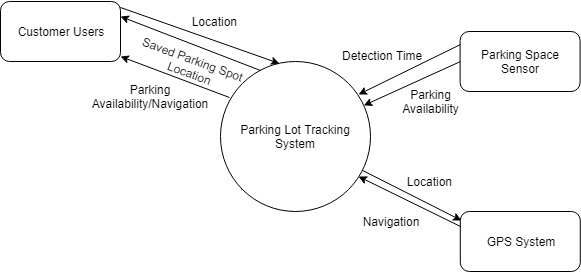
\includegraphics[width=40em]{ContextDiagram.png}
		\caption{Context Diagram - Data Flow of the System.}
		\label{fig:cd}
	\end{figure}
	\section{Component Diagram}
	\begin{figure}[H]
		\centering
		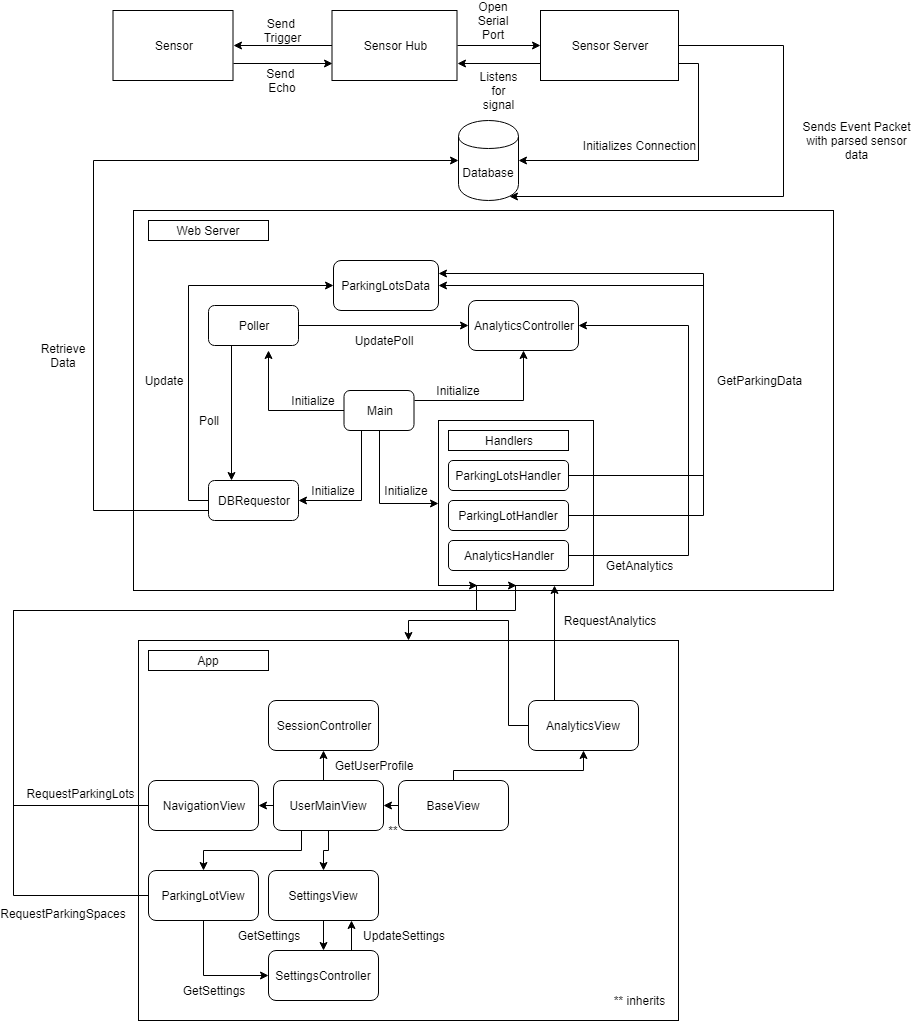
\includegraphics[width=40em]{Images/ComponentDiagram.png}
		\caption{Component Diagram for ParkMe - Interactions Between Components.}
		\label{fig:cmd}
	\end{figure}
	\section{Database Design}
	\begin{figure}[H]
		\centering
		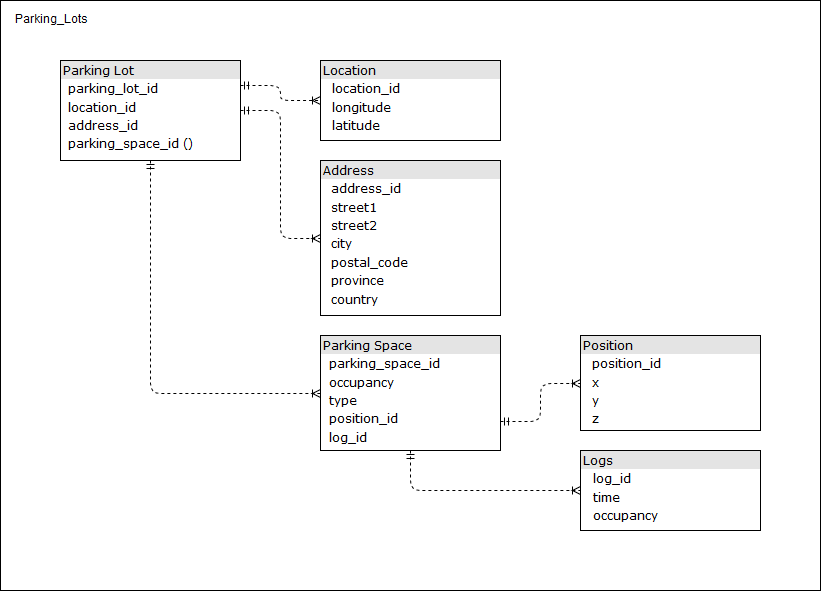
\includegraphics[width=40em]{database.png}
		\caption{Database Schema - Design of the Database.}
		\label{fig:dd}
	\end{figure}
	
	
	\section{Monitored and Controlled Variables}
	ParkMe only contains two systems where it interacts with the environment around it: The mobile application where the user interacts with our system directly and the system responds back. The parking identifier is the second system where the users only interact with it and it does not directly interact with it.
	
	\subsection{Monitored Variables}
	\begin{table}[H]
		\begin{tabular}{ | m{4cm} | m{1.5cm}| m{2cm}| m{3cm}| m{3cm} |} 
			\hline
			Name & Type & Range & Units & Physical Interpretation \\ [0.5ex] 
			\hline
			\hypertarget{SPOCC}{SPOT\_OCCUPATION} & Status & "true"/"false" & Unitless & If the Parking Spot Identifier has detected a vehicle or obstacle in the way. \\ 
			\hline
			\hypertarget{UGPSDT}{USER\_GPS\_DATA} & GPS & Longitude: -180 ,180
			Latitude: -90, 90
			& Longitude, Latitude in Degrees & The GPS location data of the users mobile device. \\ 
			\hline 
			\hypertarget{UDVCROT}{USER\_DEV\_ROTATION} & Vector2 (Number, Number) & Does not have a range & Unitless & The rotation of the mobile device relative to the normal of the device. \\
			\hline
			\hypertarget{UAIN}{USER\_APP\_INPUT} & Action & Does not have a range & Unitless & The user’s varied input to the mobile application** \\	
			\hline
		\end{tabular}
		\caption{Monitored Variables for ParkMe.}
		** - User inputs are described in the Software Requirements Specification document, this is just the general idea of inputs being registered from the environment from the user that all falls under potential application actions.
	\end{table}
	
	\subsection{Controlled Variables}
	\begin{table}[H]
		\begin{tabular}{ | m{5cm} | m{2cm}| m{1.5cm}| m{2cm}| m{3cm} |} 
			\hline
			Name & Type & Range & Units & Physical Interpretation \\ [0.5ex] 
			\hline
			\hypertarget{UNAV}{USER\_NAVIGATION} & -- & -- & -- & The navigation the application uses to guide the user to the parking lot. \\ 
			\hline
			\hypertarget{PSAVAIL}{SPOT\_AVAILABILITY} & Status & Occupied / Full & Unitless & If the parking  spot is occupied. \\
			\hline
			\hypertarget{PSTYPE}{SPOT\_TYPE} & Status & Accessible / N/A & Unitless & If the parking  spot is an  accessible type. \\
			\hline
			\hypertarget{PLSTAT}{PARKING\_LOT\_STATUS} & List of Statuses & List of True/False & Unitless & A mapping of the parking lot that the user requested with their availabilities. \\ 
			\hline 
			%\hypertarget{PLANLT}{PARKING\_LOT\_ANALYTICS} & Numbers & Varied & Varied & The statistics and trends relating to a parking lot/parking spot.** \\	
			%\hline
		\end{tabular}
		\caption{Controlled Variables for ParkMe.}
		** - User inputs are described in the Software Requirements Specification document, this is just the general idea of inputs being registered from the environment from the user that all falls under potential application actions.
	\end{table}
	
	\section{Constants}
	\begin{itemize}
		\item \hypertarget{RESPONSETIME}{FLOAT - PARKING\_SPOT\_RESPONSE\_TIME} = 500ms 
		
		\item \hypertarget{EXPTIME}{FLOAT - PARKING\_SPOT\_EXPIRATION\_TIME\_WARNING }= 10 minutes
		
		\item \hypertarget{CONCUSERS}{INT - MAX\_CONCURRENT\_USERS} = 1000 users
		
		\item \hypertarget{DETERR}{FLOAT - DETECTION\_ERROR\_RATE} = 0.01\%
		
		\item \hypertarget{NBDST}{INT - NEARBY\_DISTANCE} = 20 km
		
		\item \hypertarget{MINCAP}{INT - MINIMUM\_ALLOWED\_CAPACITY} = 150 MB
	\end{itemize}
	
	\section{Behaviour Overview}
	\textit{The following is taken from the Software Requirement Specifications Rev. 1 document.}\\\\
	To solve the problems mentioned above, Park Me will implement several general systems. The first and most important of these is the ability to monitor the occupancy of parking spots in a given parking area through a series of physical sensors. This data will then be used by the mobile application to update the customer on the number of available spots in the lot, as well as the location of those spots. Specific data on information such as accessible parking, expectant mothers, paid parking...etc will also be displayed, and will utilize preferences set by the user.  \\
	
	Ideally, the application will also include functionality to navigate the user to a parking spot/row/area, but this integration will depend on the accuracy and availability of GPS systems and the complexity of those systems.
	
	
	\section{Component Breakdown}
	\subsection{Sensor Component (Module-HW-S)}
	\begin{itemize}
		\item \textbf{Input/Output:} Each sensor will have a voltage, ground, and trigger input, as well as a data output.
		\item \textbf{Behaviour Description:} Each sensor will take in power inputs, and a trigger input that instructs it to take in its sensor data. The collected data will then be output through the hardwired connection to the sensor hub.
		\item \textbf{Timing Constraints/Performance Requirements:} Each sensor must continually maintain a data connection and provide constant real-time information to the sensor hub such that its error detection rate is less than \hyperlink{DETERR}DETECTION\_ERROR\_RATE.
		\item \textbf{Initialization:} Not applicable for purely hardware peripherals.
	\end{itemize}
	
	\subsection{Sensor Hub Component (Module-HW-A)}
	\begin{itemize}
		\item \textbf{Input/Output:} The Sensor Hub Component will take in sensor data as input, and output final sensor information to the serial port.
		\item \textbf{Behaviour Description:} The sensor component will input data to the Sensor Hub Component, which will then clean the data and format a data packet with time, sensor reading, and sensor identifier. This formatted packet will be sent through serial port to the sensor server component.
		\item \textbf{Timing Constraints:} The sensor component must continually receive data in real time and push the formatted packets to the serial port immediately.
		\item \textbf{Initialization:} The sensor component will be initialized with the sensor pin assignments, sensor thresholds, as well as the serial port opening.
	\end{itemize}
	
	\subsection{Sensor Server Component (Module-HW-P)}
	\begin{itemize}
		\item \textbf{Input/Output:} The Sensor Server component will receive serial port data and will output server data updates with the new information.
		\item \textbf{Behaviour Description:} The component will take in serial port data which consists of formatted packets of sensor information, and will format the data further to fit the database schema. The component will then update the database entry for the sensor with the new data.    
		\item \textbf{Timing Constraints:} The Sensor Server component will need to maintain a real-time connection to the serial port and format the data in real time as well. In addition to this, it will need to generate the database update requests and send them in real time.
		\item \textbf{Initialization:} The Sensor Server component will be initialized with a serial port connection, as well as a connection to the database server.
	\end{itemize}
	
	\subsection{Database Component (Module-DB)}
	\begin{itemize}
		\item \textbf{Input/Output:} The database component is a database instance that receives and sends data to the server.
		\item \textbf{Behaviour Description:} The database receives data inputs from the server and updates the document belonging to the parking lot collection. Each document contains information about a parking spots availability and status and sends this information back to the server when requested.
		\item \textbf{Timing Constraints:} The database component should contain the most up to date status for each parking spot. The database should also always be running and ready to receive updates in real time.
		\item \textbf{Initialization:} The database component will be initialized with a predetermined schema where each collection and document pairs will use the same data types.
	\end{itemize}
	
	\subsection{Web Server}
	\begin{itemize}
		\item \textbf{Input/Output:} The web server will receive API RESTful requests from the mobile application and will be responsible for returning RESTful responses back.
		\item \textbf{Behaviour Description:} The server will be responsible for supplying the parsed database data to the mobile application. This server will act as a middle ground between the mobile application and the database to ensure security and force a single point entry for the database. It will also be responsible for computing the real-time analytics as well as supplying this data to the mobile application.
		\item \textbf{Timing Constraints:} The server should supply data that is update to date with reference to the requirements laid out in the Software Requirement Specifications document Rev 1. Additionally the server should not ever stop running so that all API requests are successfully returned.
		\item \textbf{Initialization:} The server will be started up/initialized once to allow for its subcomponents to initialize as well.
	\end{itemize}
	\textbf{Sub-Components:}
	
	
	\subsubsection{Main (Module-SW-M)}
	Starts up the server and initializes all connected components.
	
	\subsubsection{Poller (Module-SW-P)}
	\begin{itemize}
		\item \textbf{Input/Output:} Gets initialized from the Main component, and updates the AnalyticsController on poll event.
		\item \textbf{Behaviour Description:} Continually retrieves calls database to update local server data storage as well as updates the AnalyticsController with update to date data.
		\item \textbf{Timing Constraints:} The poller runs at a frequency determined the Software Requirement Specifications document.
		\item \textbf{Initialization:} Initializes the poller frequency based on requirement specifications.
	\end{itemize}
	
	\subsubsection{DBRequestor (Module-SW-DB)}
	\begin{itemize}
		\item \textbf{Input/Output:} Gets called from the Poller component, and updates the ParkingLotsData component with requested data from database.
		\item \textbf{Behaviour Description:} Requests the updated data from the database and sends to ParkingLotsData component to perform analytics on.
		\item \textbf{Timing Constraints:} The poller runs at a frequency determined the Software Requirement Specifications document.
		\item \textbf{Initialization:} Initializes a connection to the database.
	\end{itemize}
	
	\subsubsection{AnalyticsController (Module-SW-AC)}
	\begin{itemize}
		\item \textbf{Input/Output:} Retrieves data from the ParkingLotsData component and gets requested analytics from both ParkingLotsHandler and ParkingLotHander.
		\item \textbf{Behaviour Description:} Performs analytic computations on data storage held in ParkingLotsData.
		\item \textbf{Timing Constraints:} The AnalyticsController should update its analytics whenever the ParkingLotsData component is updated with new data.
	\end{itemize}
	
	\subsubsection{ParkingLotsHandler (Module-SW-PLSH)}
	\begin{itemize}
		\item \textbf{Input/Output:} Retrieves API requests from mobile application and returns the appropriated RESTful response.
		\item \textbf{Behaviour Description:} Handles all API that has to do with all the parking lots in the system.
		\item \textbf{Timing Constraints:} The requests should respond as fast as the Software Requirement Specifications document has specified.
		\item \textbf{Initialization:} The handler will be initialized and hook into API endpoints on start up.
	\end{itemize}
	
	\subsubsection{ParkingLotHandler (Module-SW-PLH)}
	\begin{itemize}
		\item \textbf{Input/Output:} Retrieves API requests from mobile application and returns the appropriated RESTful response.
		\item \textbf{Behaviour Description:} Handles all API that has to do with a specific parking lot.
		\item \textbf{Timing Constraints:} The requests should respond as fast as the Software Requirement Specifications document has specified.
		\item \textbf{Initialization:} The handler will be initialized and hook into API endpoints on start up.
	\end{itemize}
	
	\subsubsection{AnalyticsHandler(Module-SW-AH)}
	\begin{itemize}
		\item \textbf{Input/Output:} Retrieves API requests from mobile application and returns the appropriated RESTful response.
		\item \textbf{Behaviour Description:} Handles all API that has to do with any analytics provided in the system.
		\item \textbf{Timing Constraints:} The requests should respond as fast as the Software Requirement Specifications document has specified.
		\item \textbf{Initialization:} The handler will be initialized and hook into API endpoints on start up.
	\end{itemize}
	
	\subsubsection{ParkingLotsData (Module-SW-PLD)}
	\begin{itemize}
		\item \textbf{Input/Output:} Gets updated by the DBRequestor component and provides parsed data to the AnalyticsController as well as the ParkingLotHandler and ParkingLotsHandler.
		\item \textbf{Behaviour Description:} Handles all manipulation (getters/setters) of the data copied from the database into the server.
		\item \textbf{Timing Constraints:} The requests should respond as fast as the Software Requirement Specifications document has specified.
		\item \textbf{Initialization:} It will be initialized on startup and continually updated with the polling DBRequestor component.
	\end{itemize}
	
	
	\subsection{App}
	\begin{itemize}
		\item The app will be responsible for interpreting the parsed database data and displaying it in a way understandable and informative to users. This app will act as an interface between users and the server to aid in information retrieval and understanding. It will also be responsible for displaying the real-time analytics, navigation, and parking lot mappings to the user so they can interactively but abstractedly send requests to the server.
		\item \textbf{Timing Constraints:} The app should supply data that is update to date with reference to the requirements laid out in the Requirements Document Rev 1.
		\item \textbf{Initialization:} The app will be started up/initialized upon each new session (app has been fully exited previously) to allow for its session controller and base component to initialize as well.
	\end{itemize}
	\textbf{Sub-Components:}
	
	\subsubsection{Base (Module-SW-S-BV)}
	\begin{itemize}
		\item \textbf{Input/Output:} Starts up application initialization.
		\item \textbf{Behaviour Description:} Initializes base application function. Displays landing page for application, and user mode selection.
		\item \textbf{Timing Constraints:} The startup should respond as fast as the Software Requirement Specifications document has specified.
		\item \textbf{Initialization:} Initializes a connection with the server.
	\end{itemize}
	
	\subsubsection{UserMain (Module-SW-S-UMV)}
	\begin{itemize}
		\item \textbf{Input/Output:} Gets initialized from BaseView. Initializes and updates SessionController and SettingController, updates interface for all functionality available to the user when in UserMain mode.
		\item \textbf{Behaviour Description:} Displays functionality of user mode as described in the Software Requirement Specifications document. Allows user to input a location and returns nearby parking lots. Makes requests to the server for possible parking lots.
		\item \textbf{Timing Constraints:} The requests should respond as fast as the Software Requirement Specifications document has specified.
		\item \textbf{Initialization:} Initializes the SettingsController and SessionController.
	\end{itemize}
	
	\subsubsection{Settings (Module-SW-S-SV)}
	\begin{itemize}
		\item \textbf{Input/Output:} Gets initialized by request from UserMainView. Sends settings API requests.
		\item \textbf{Behaviour Description:} Handles all settings API requests (getters/setters) to modify current user settings and preferences.
		\item \textbf{Timing Constraints:} The requests should respond as fast as the Software Requirement Specifications document has specified.
		\item \textbf{Initialization:} Hooks into the session and settings controllers.
	\end{itemize}
	
	\subsubsection{SessionController (Module-SW-S-SSC)}
	\begin{itemize}
		\item \textbf{Input/Output:} Gets initialized from the UserMainView. Allows access and change of current user parking status, and location.
		\item \textbf{Behaviour Description:} Handles user parking lot space state for later retrieval and navigation.
		\item \textbf{Timing Constraints:} The requests should respond as fast as the Software Requirement Specifications document has specified.
		\item \textbf{Initialization:} Initialized on UserMainView startup and hooks into UserMainMenu.
	\end{itemize}
	
	\subsubsection{SettingsController (Module-SW-S-SEC)}
	\begin{itemize}
		\item \textbf{Input/Output:} Gets initialized from the UserMainView. Allows access and change of current user preferences for spot location, type, etc.
		\item \textbf{Behaviour Description:} Handles user preferences for the session, allowing for modification and retrieval via API requests.
		\item \textbf{Timing Constraints:} The requests should respond as fast as the Software Requirement Specifications document has specified.
		\item \textbf{Initialization:} The controller will initialize and hooks into SettingsView and UserMainMenu.
	\end{itemize}
	
	\subsubsection{NavigationView (Module-SW-S-NV)}
	\begin{itemize}
		\item \textbf{Input/Output:} Gets initialized from UserMainMenu. Sends maps API request constructed from UserMainMenu, once user has chosen a parking lot location. Displays the returned navigation info, alongside verbal instructions.
		\item \textbf{Behaviour Description:} Provides navigation instructions to the user’s previously selected parking lot, both visually and verbally, using pre-existing APIs.
		\item \textbf{Timing Constraints:} The poller runs at a frequency determined the Software Requirement Specifications document.
	\end{itemize}
	
	\subsubsection{ParkingLotView (Module-SW-S-PLV)}
	\begin{itemize}
		\item \textbf{Input/Output:} Gets initialized from UserMainMenu. Sends/receives request to server to get ParkingLot info, once user has chosen a parking lot location from the UserMainMenu. Requests preferences from SettingsController and sends spot info to UserMain.
		\item \textbf{Behaviour Description:} Suggests available parking spots based on UserSettings and displays location and approximate user location, for navigation, once the user has reached the parking lot.
		\item \textbf{Timing Constraints:} The requests should respond as fast as the Software Requirement Specifications document has specified.
	\end{itemize}
	
	\subsubsection{AnalyticsView (Module-SW-S-AV)}
	\begin{itemize}
		\item \textbf{Input/Output:} Gets initialized from the baseView. Displays graph data via API usage, sends requests to the server.
		\item \textbf{Behaviour Description:} Displays graphs and other analytics as available.Makes requests to the server for required parsed database data then displays it as specified.
		\item \textbf{Timing Constraints:} The requests should respond as fast as the Software Requirement Specifications document has specified.
	\end{itemize}
	
	\section{Normal Operation}
	The normal operation sequence of the system is as follows.
	\begin{itemize}
		\item The sensors take in data from parking spaces.
		\item The sensor component receives the sensor data, formats it, and then sends it through the serial port.
		\item The Sensor Server component continually reads the serial port for update packets, formats them to follow database schema, and then sends the update request to the database.
		\item The database updates the respective tables.
		\item The mobile application pulls database data and provides an interface for users.
	\end{itemize}
	
	\section{Undesired Event Handling}
	\textit{The following is taken from the Software Requirement Specifications Rev. 1 document.}\\\\
	In the event of a undesired event that is not a result of a previously stated assumption, the system will be designed in such a way that it will self-correct any discrepancies. This means that any desynchronization issues between the application and the servers will be fixed with the use of multiple users supplying data to the database. Additionally this will be solved by having periodic updates so that the most recent data is used. Finally, in the case of an undesired event that is not covered, the use of error handling and error messages will be utilized to prevent any confusion for the user and preventing any disastrous errors within the system.
\end{document}
